%
% conclusions and summary tables about timeline and budget
%
% Author: Michele Punturo ...
% Version:
%
%
%
The evolution toward the Einstein Telescope observatory has been, is and will be a long path.  In the following subsections we will try to depict a possible roadmap for the realisation of the observatory and we will present a first budget of the project. 
%
\subsection[ET Timeline]{ET project timeline}
%
\label{TimelineSubSection}
The idea of a third generation GW detector born within the ILIAS project (\url{http://www-ilias.cea.fr/}, 2004--2008), supported by the European Commission within the Framework Programme 6 (FP6). In fact in that ``Integration Activity'', both a ``Joint Research Activity'' (JRA3 or ``STREGA''), supporting R\,\&\,D  activities addressed to the thermal noise reduction, and a networking activity (N5-WP3), addressed to the studies for the third generation of GW detectors, have been implemented.  On the same period, a first proposal (under FP6) for a ``generic'' design study for a third generation GW detector failed for lack of funding.  
In 2005, the European Science Foundation (ESF) supported an  ``Exploratory Workshop'' (\url{http://esf-gw.pg.infn.it/}) specifically devoted to an European third generation GW observatory. This has been the right kick-off meeting to prepare the organization and clarify the targets of the successful proposal that bring to  the funding, by the European Commission, under FP7, of the ET conceptual design study, object of this document. 
\par
The main target of this conceptual design, as mentioned in Sec.~\ref{Prologue}, is the demonstration of the feasibility of the ET project, through the definition of the requirements and main characteristics of the hosting site, the design of the key components of the research infrastructure, the indication of the possible technologies and the presentation of the detector design main elements. A rough cost evaluation is then reported to evaluate the financial feasibility of the ET project.
\par 
After the conceptual design phase, a series of difficult steps are expected. 
The first step is the consolidation of the design solving the several question marks currently present in many technologies needed for ET. In fact the detectors in the ET observatory will adopt technologies that aren't explored in the advanced detectors, like cryogenics, Silicon mirrors, different wavelength lasers, optical squeezing, gravity gradient noise subtraction techniques. The ET design consolidation needs, then, an intense R\,\&\,D activity devoted to these technologies. The ET community must find the (human and financial) resources  to support these activities; these resources  should be a mix of national and international funds (i.e.\ like the ASPERA R\,\&\,D funds).   In parallel to the progresses of the technologies, the conceptual design needs to evolve in a technical design, describing in detail the components of the observatory.
This phase of the project will need a correct framework and, because of the fact that the national funding agencies in Europe are fully engaged with the realisation of the advanced detectors, a possible choice is a networking or integration tool at European level (probably in FP8). 
To support this phase and to give a future to the ET project is, then, strongly recommended to inserted it in the list of the major research infrastructures (the so--called ESFRI roadmap) recommended by the ``European Strategy Forum on Research Infrastructures'' (ESFRI). Already part of the activities, necessary to achieve this target, has been performed inserting ET in the specialised roadmaps, like the GWIC roadmap (Fig.~\ref{Fig:Roadmap} or \url{https://gwic.ligo.org/roadmap/}) and the ASPERA roadmap \url{http://www.aspera-eu.org/images/stories/files/Roadmap.pdf}, but intense outreaching and proposition actions are still needed. In Fig.~\ref{Fig:Roadmap} the worldwide roadmap for the GW detectors, produced by GWIC, is shown; although it is a bit obsolete, being produced before the outcomes of this design study, it is useful to show the overall scenario where the ET project will evolve. In the Fig.~\ref{Fig:ET-Roadmap} the expected steps of the ET project are shown, as elaborated within this conceptual design. Hence, after the current conceptual design, as previously mentioned, a technical design phase, supported by an intense R\,\&\,D activity, is necessary. Then the ET project will need to define the best site location and to start a funding search activity. An \emph{a priori} condition for the funding of the construction phase is the detection of a GW signal in the advanced detectors. To base the ET construction funding and start-up on a so intrinsically  unpredictable event seems rather hazardous, but considering the  installation and commissioning schedule of the advanced detectors and  the promised sensitivity evolution, it is possible to predict a realistic time window for the GW signal from a BNS system in the 2015--2017 period. 
It will follow a site preparation phase, where all the legal and preliminary aspects of the land ownership acquirement are exploited. In parallel the production and test of the first detector hardware components will start in the laboratories participating to the ET project. The site and infrastructures realisation will last for about four years, followed by the first ET detector installation. To save time, it is expected that part of the first detector installation (i.e.\ vacuum pipes deployment) could overlap with the latest infrastructure realisation activities. 
Thanks to the experience acquired with the initial GW detectors (that will be improved with the next commissioning of the advanced interferometers) it is possible to state that the commissioning phase will last at least for more than 3--4 years, with some early science data taking interlaced with the commissioning periods. 
\par 
The ET observatory infrastructures and detectors are designed having as requirement the modularity of the components; this will allow sequential installation phases, interlaced with periods of data taking for the detectors, already operative in the ET site. In this way it will be also possible to upgrade the installed detectors when the technological progresses will make it convenient, maximising the duty cycle. This possibility underlines the main target of this study: to provide the design of a Research Infrastructure operative for decades and will be able to host evolving detectors.
%
\FloatBarrier
\begin{figure}[hthp!]
%\includegraphics[width=1.0\textwidth, bb=0 0 800 600]{Sec_Conclusions/Roadmap.png}
%\includegraphics[width=1.0\textwidth]{Sec_Conclusions/Roadmap.png}
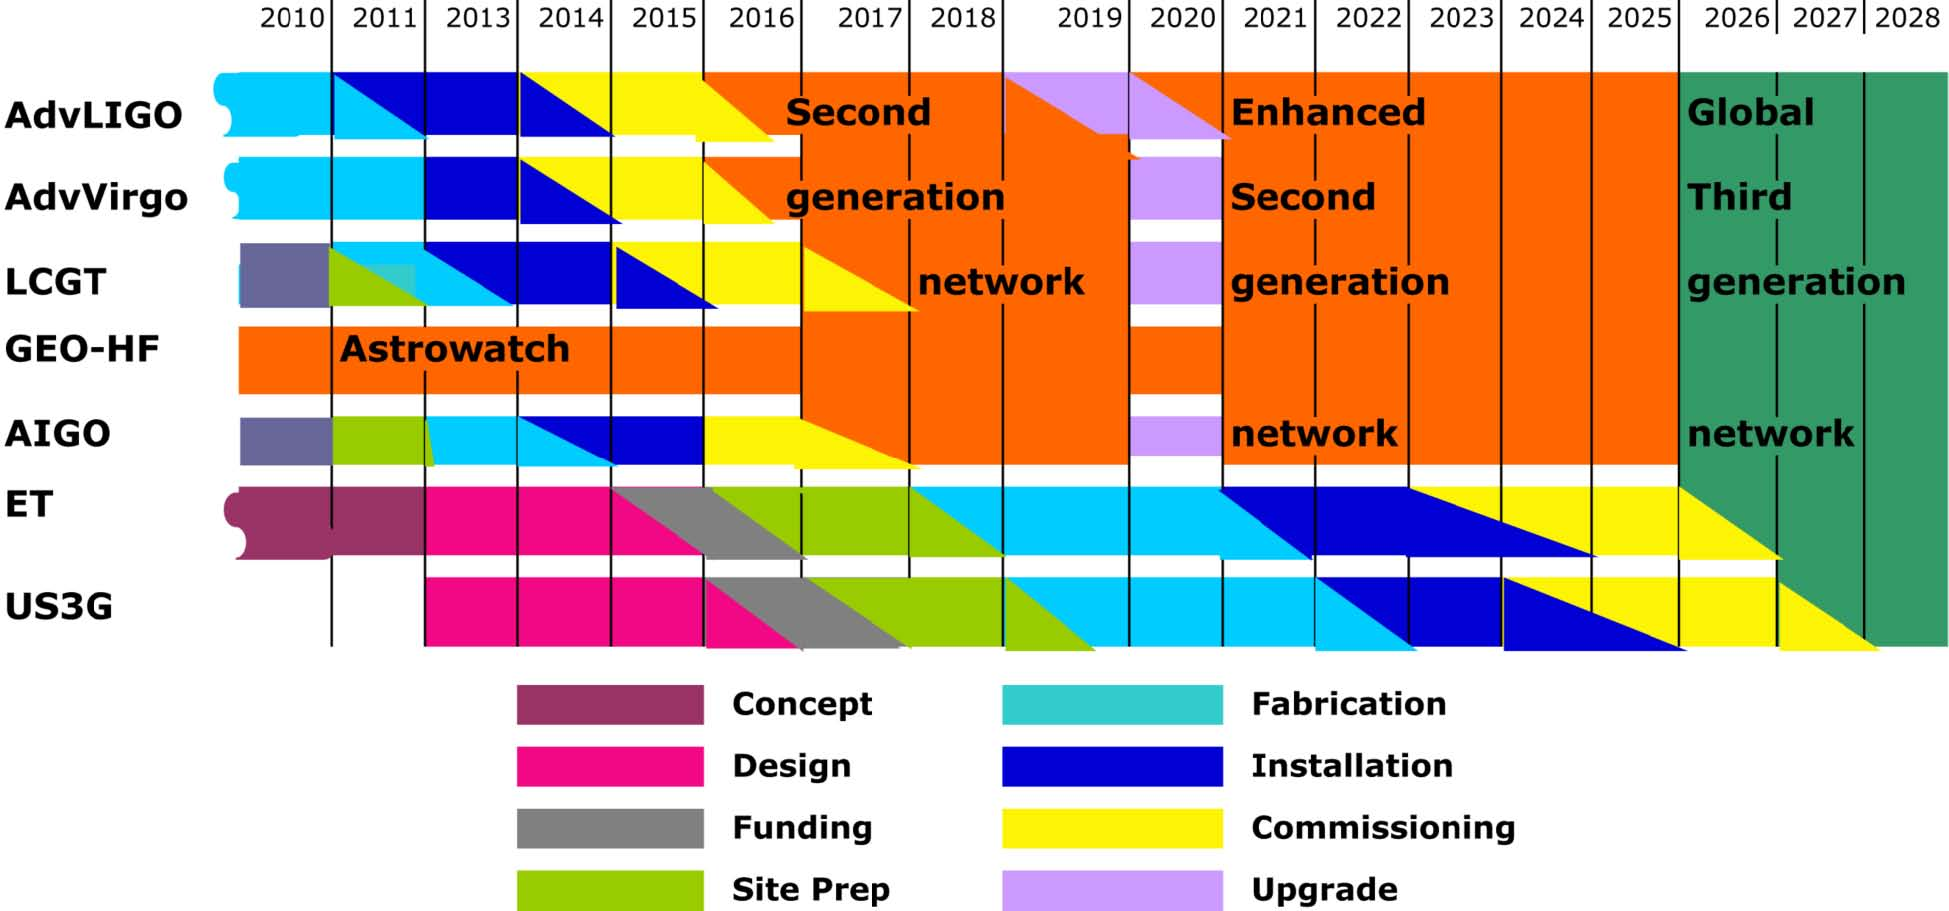
\includegraphics[width=1.0\textwidth]{Sec_Conclusions/Roadmap_GWIC_rev30_1.jpg}
% figure caption is below the figure
\caption{GWIC roadmap (rev.~$30.1$) showing the evolution of GW detectors in the World. The absolute timing for ET, shown in this figure, is a bit obsolete, being it produced before this design study}
\label{Fig:Roadmap}       % Give a unique label
\end{figure}
%
%
\FloatBarrier
\begin{figure}[hthp!]
%\includegraphics[width=1.0\textwidth, bb=0 0 800 600]{Sec_Conclusions/Roadmap.png}
%\includegraphics[width=1.0\textwidth]{Sec_Conclusions/Roadmap.png}
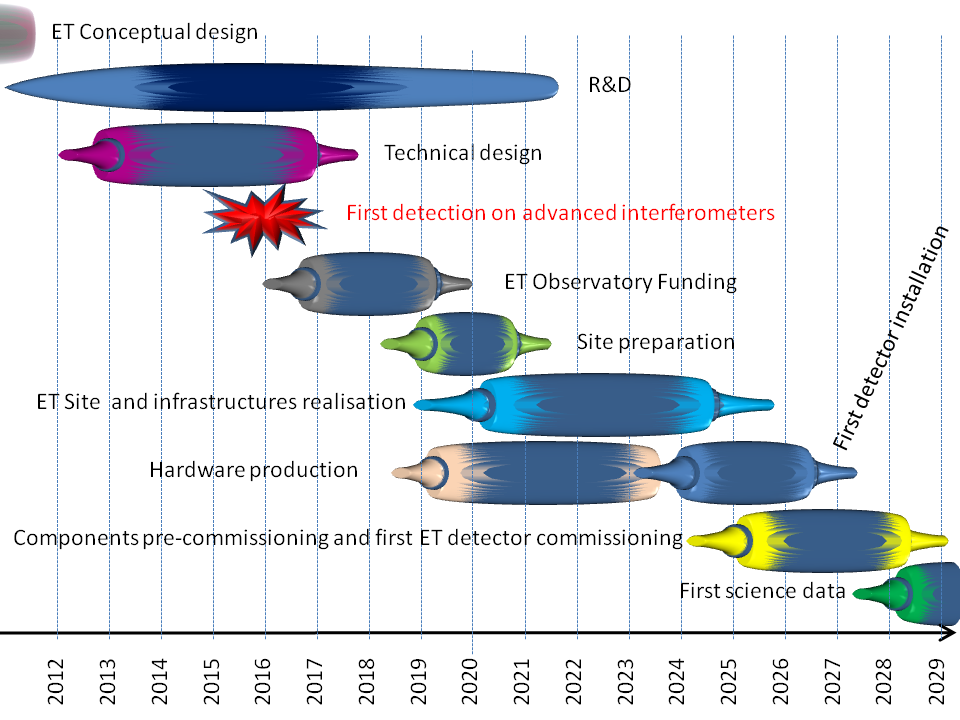
\includegraphics[width=1.0\textwidth]{Sec_Conclusions/ET-roadmap.png}
% figure caption is below the figure
\caption{ET expected timeline. The incertitude in the start-stop of each activity is pictorially represented through the lateral appendixes to each horizontal bar.}
\label{Fig:ET-Roadmap}       % Give a unique label
\end{figure}
%
%
\subsection[ET costs]{ET project preliminary cost evaluation}
%  
\label{ConclusionsCostsSubSection}
%
One of the main targets of this conceptual design study is a rough evaluation of the costs of the ET observatory. The level of detail of this document is not studied to provide a detailed cost table of the whole project, being this one of the deliverable of the technical design phase, but a cost evaluation, for each macro-systems composing the ET observatory, is provided. 
%
In table~\ref{Fig:TotalCostTable} the cost summary and the time distribution of the expenditures are shown, whereas in the following sections the cost evaluation is divided in to the five ET macro-systems. .
%
\FloatBarrier
\begin{figure}[hthp!]
\centering 
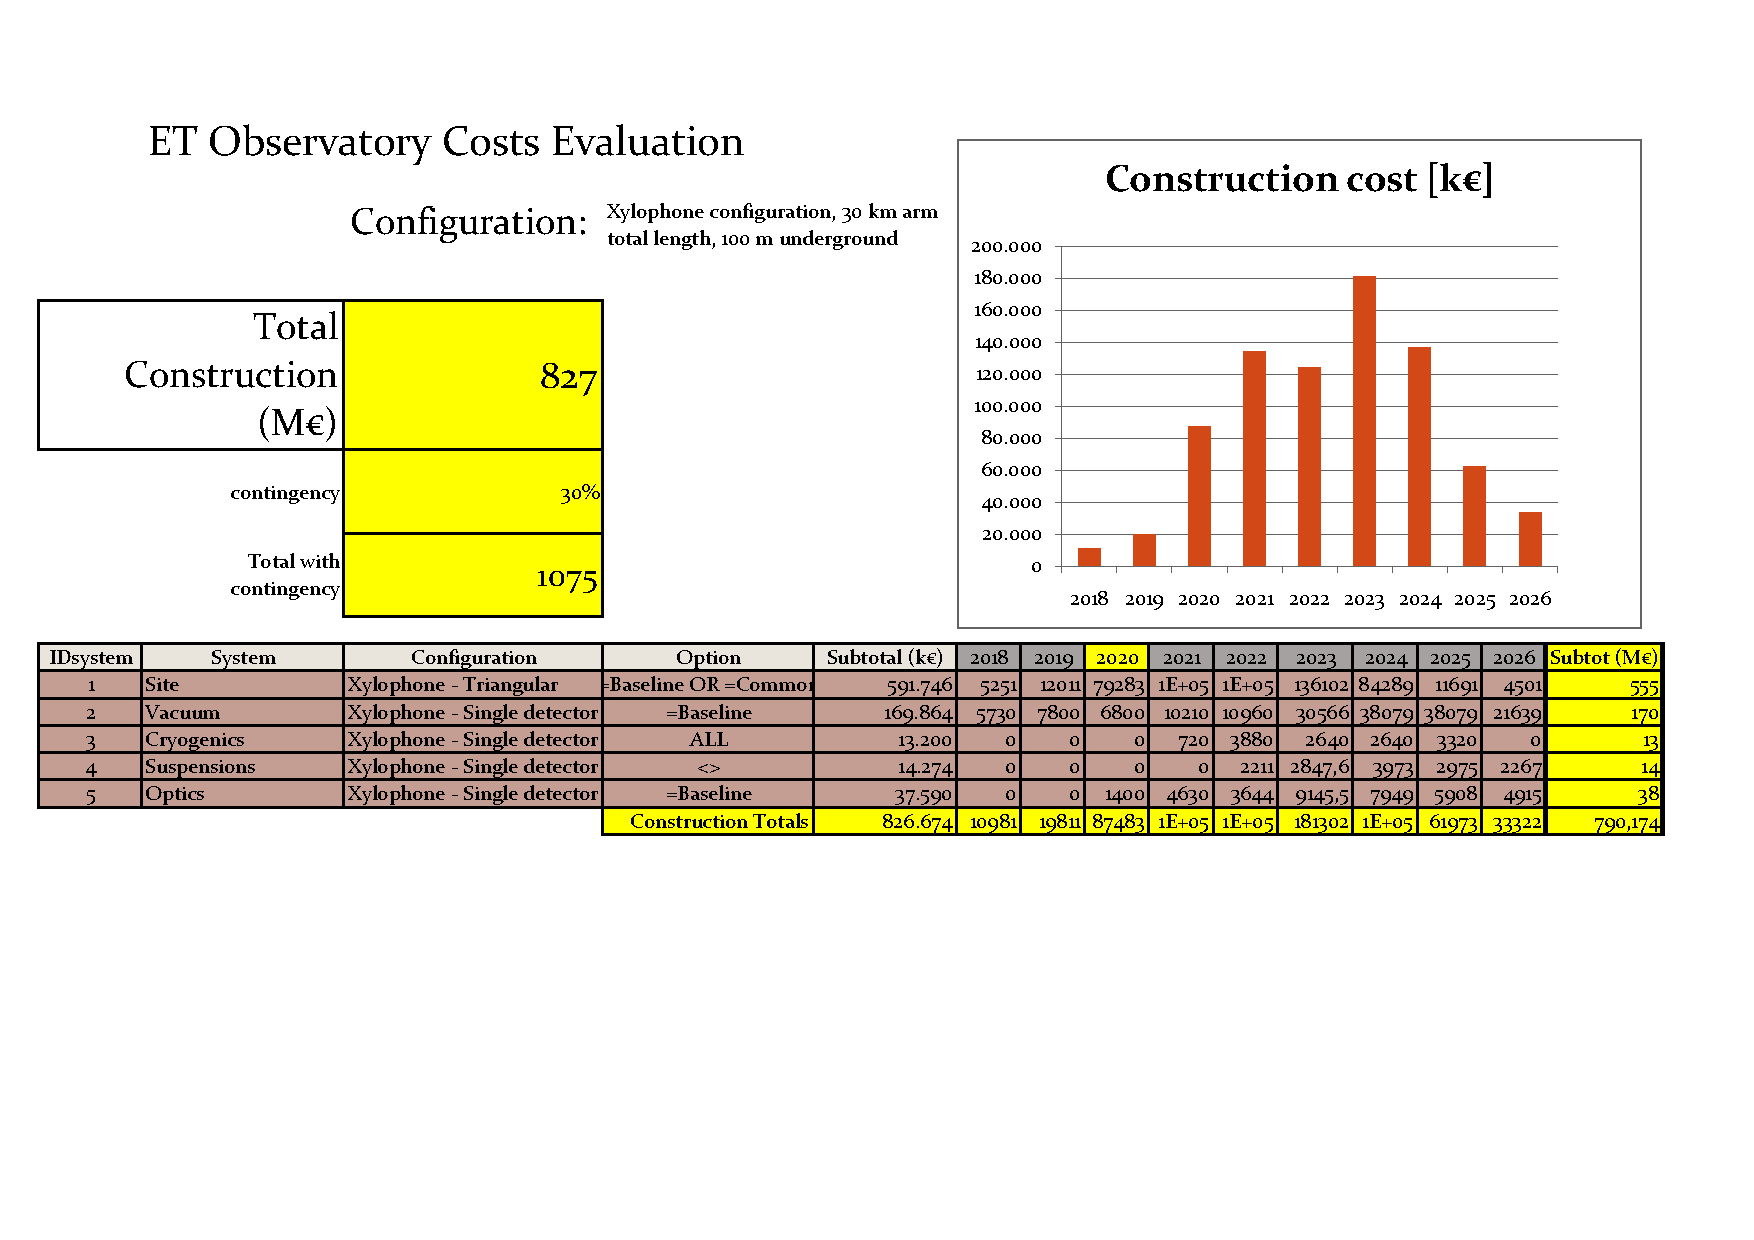
\includegraphics[angle=90, width=0.5\textwidth]{Sec_Conclusions/ET-cost-v00r05-Total.pdf}
%
%%\includegraphics[angle=90, width=1.0\textwidth]{Sec_Conclusions/ET-cost-v00r02.pdf}
%\includegraphics[width=0.49\textwidth, bb=0 0 800 600]{ET-B.png}
\caption{ET observatory cost summary and expenditure time distribution}
\label{Fig:TotalCostTable}
\end{figure}
%
%
%
\subsubsection[Site costs]{Infrastructure cost preliminary evaluation}
%  
\label{ConclusionsSiteCostsSubSection}
%
The total estimated value for the infrastructure costs is 775 MEuro (in 2011 \euro). The cost is determined for a single xylophone detector mode. This configuration constitutes the phase I instrumentation of the project. Phase II will be realized later and features a triple xylophone interferometer configuration.

The site specific costs are related to the direct costs for providing the infrastructure to site the observatory and are estimated at 592 MEuro (2011 value level). These costs include the underground civil facilities, services (electricity and water distribution), buildings and surface construction. The actual site-specific costs will depend on the location where the observatory is constructed, and the facilities that already exist at that location. For the estimates we have used 260 \euro $/ \mathrm{m^3}$ for the excavation costs. This includes digging cost, soil transportation and deposit, and finishing the floor and cavern walls with concrete. In addition, construction machines, running cost, maintenance, preparation and management costs are included. Several underground sites in Europe have been identified that comply with such costs, although a significant bandwidth applies. The number is also compliant with the site costs for LCGT in Japan.

The infrastructure costs include the direct costs for the safety and security systems, cooling and ventilation systems. Cost of the vacuum system and the cryogenic infrastructure are presented elsewhere. These costs are based on both the experience at GEO, Virgo and worldwide tenders.
 

A breakdown is given in Fig.~\ref{fig:etcost2}. It is apparent that the main cost drivers are the underground site infrastructure: tunnels and caverns. 
\FloatBarrier
\begin{figure}[htbp]
	\begin{center}
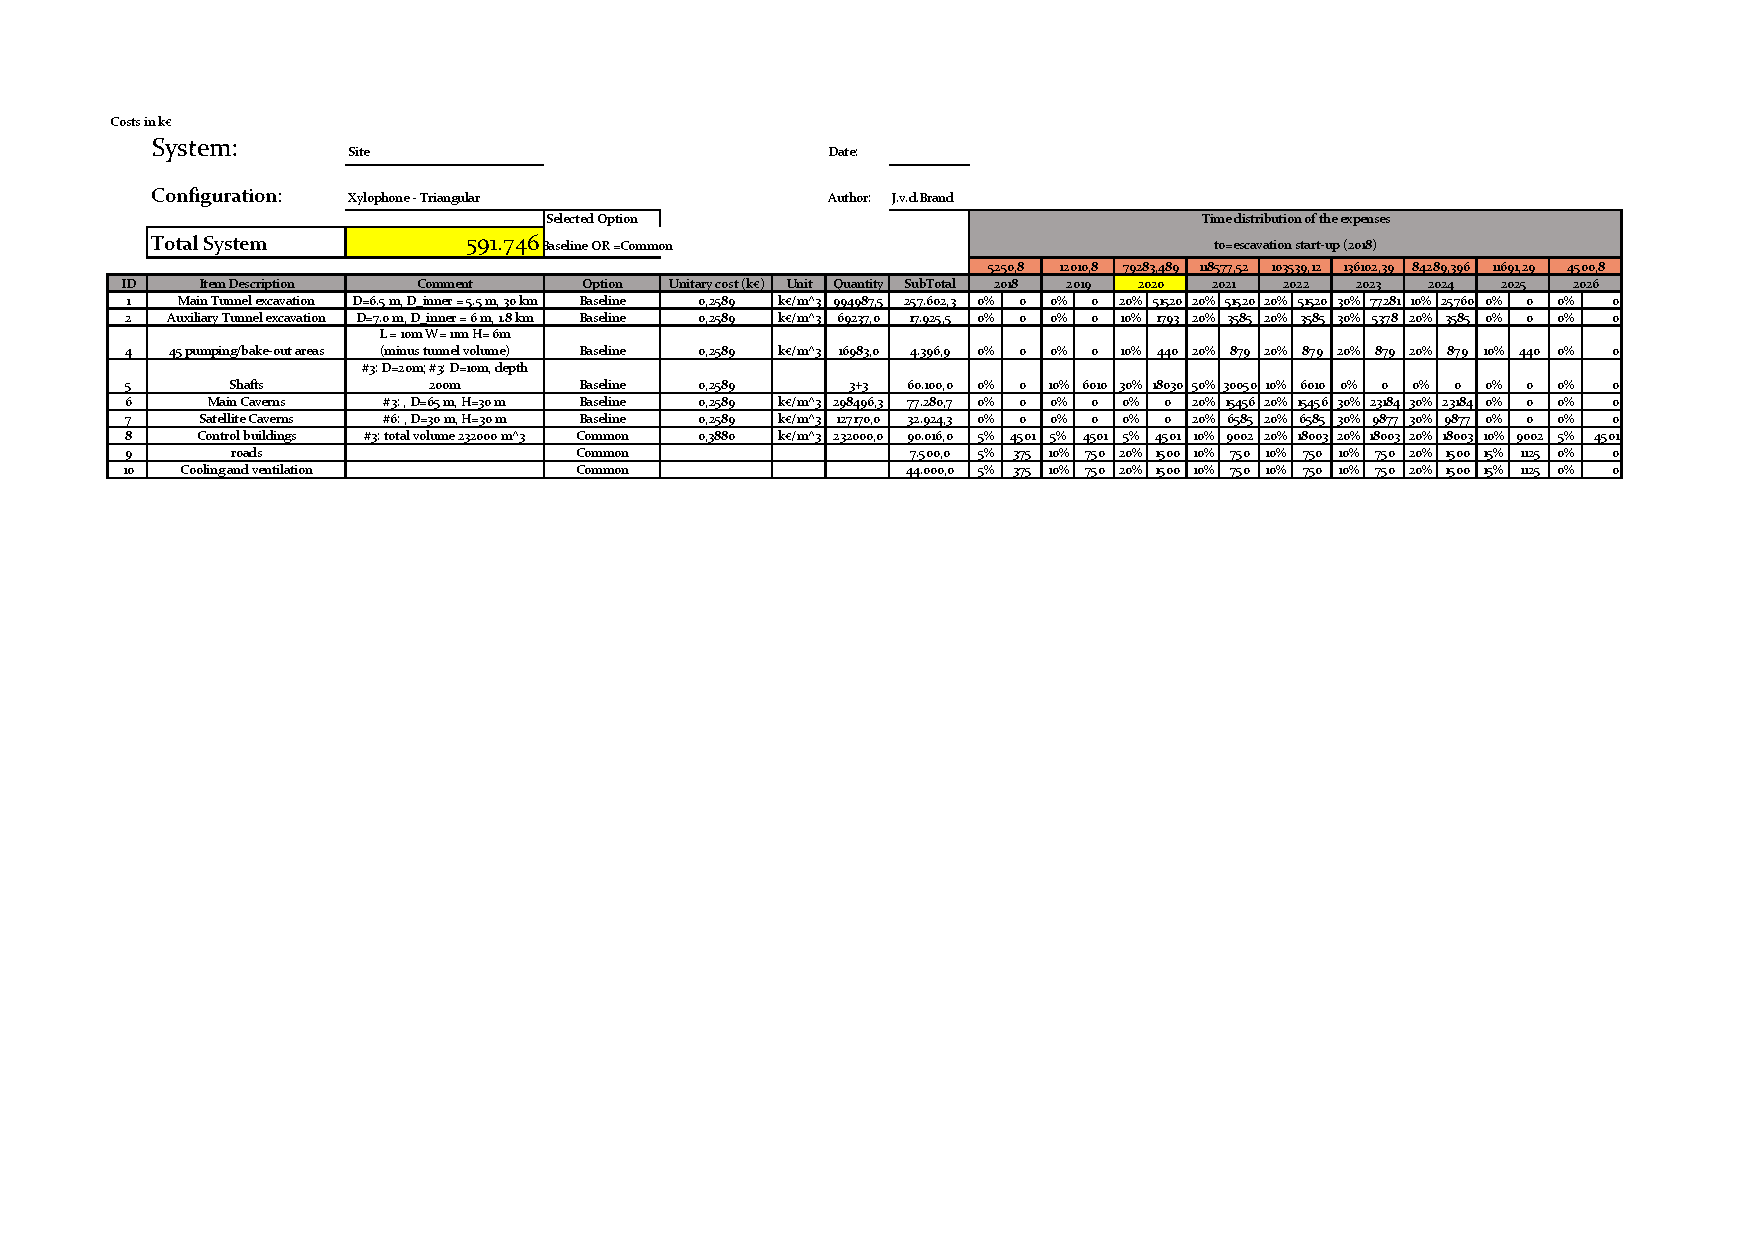
\includegraphics[angle=90, width=0.25\textwidth]{Sec_Conclusions/ET-cost-v00r05-Site.pdf}		\caption{Partitioning of the site specific costs of the Infrastructure Reference Design for phase I of the Einstein Telescope observatory.}
		\label{fig:etcost2}
	\end{center}
\end{figure}

The observatory features more than 31 km of tunnel for housing the interferometers and their filter cavities. Each corner station has a main cavern and two satellite caverns that are connected by twin tunnels. The observatory will house one main site and two satellite sites. Surface buildings will be constructed at all sites and include control rooms, conference rooms, computing center, lunch area, science education center, cleanroom facilities, office buildings, mechanical and electronics workshops, air condition buildings, storage buildings, library, and auditorium. The main site will be fenced and guarded, and will have a visitor check in facility. Depending on the site, local lodging accommodation may be considered.

Services such as cooling and ventilation are of industrial standard type. However, there are several unusual constraints as humidity and temperature stability in underground areas that represent an engineering challenge. The dense stacking of equipment in precious underground space is a further consideration. Heat dissipating objects ($e.g.$ cryogenic compressors, electronics) employ primary cooling water. All heat from the underground facilities must be rejected to the atmosphere through cooling towers. Other fluid networks involve drinking water, fire fighting water and seepage and waste water. With regard to ventilation air, the tunnels themselves are used as ducts. The system and quantity of air circulation must be optimised from the view of energy consumption. Low air flow is beneficial for noise reduction and for minimizing thermal effects. 

Safety and security systems are crucial for personal safety and disaster prevention. Various causes of disasters must be considered ($e.g.$ fires, electric power failure, cryogenic gas leaks, earthquake, terrorism). In all cases evacuation of personnel is required. Consequently, it is important that distances to safe places are minimized and that personnel is protected for several hours until rescue teams arrive. Emergency facilities must be carefully designed. Disaster prevention facilities include systems with emergency phones, emergency alarms, and fire alarms. Equipment such fire extinguishers, fire hydrant and water spray must be implemented. There has to be an active program of refuge instruction: evacuation routing, smoke facilities, and emergency illumination. A camera monitoring system must be implemented. While safety regulations are well established in law for surface facilities, this is not regulated by law in all countries for underground spaces (except in case of mining). In some cases special laws are established.

Site requirements that impact construction cost must be considered. These include topography and geological subterranean conditions. Factors such as horizontal versus vertical access to the underground facilities greatly affect the construction costs. Site availability and acquisition cost can vary greatly. Availability of existing support infrastructure is important. Underground laboratories as Laboratorio Nazionali del Gran Sasso LNGS (Italy), Laboratoire Souterrain de Mondane LSM (France), Laboratorio Subterraneo de Canfranc LSC (Spain) and Institute for Underground Science, Boulby mine (UK) provide extensive facilities for scientific and technical staff. This includes accommodations for resident staff (housing, schools, $etc.$), and visiting staff (lodging, transportation, $etc$.). For the same reason active or closed down mines may provide valuable facilities such as hosting shafts, electrical infrastructure, water pumps, and safety systems. In addition, they may provide local technical support and experienced technical staff. Other factors that determine the (cost of ) the main infrastructure design include groundwater conditions, hydrology and drainage which have an impact on the design of buildings and tunnels, accessibilities such as roads, railroad, distance to nearby supporting technical facilities, site utilities installations as power, water, and sewage. Finally, labour cost and proximity of soil waste and borrow areas must be considered. 

Aside from construction costs, there are various factors impart the operation cost. These include the cost of electrical power, cost of local labour, heating and cooling requirements, maintenance, and travel time and cost for visiting staff. Environmental, health and safety plans must be put in place to assure the safety ofusers, staff and visitors to the Einstein Telescope observatory. These plans must comply with the relevant governmental and European standards and regulations. It is important to elevate the life-safety level above that in the mining and underground construction industries to one appropriate for researchers, students, and the public. 

Risk must be minimized in the realization of the observatory. Risk factors include acquisition risk, risk from environmental sources such as earthquakes, floods and storms. Special attention must be paid to potential future man-made noise and vibration from development or industrial projects. 

The explicit labor required to realize the construction project is estimated at xx million person-hours. It includes administration and project management, installation and testing. Part of the labor will be contracted and part will come from existing labor in collaborating institutions.
%
%
\subsubsection[Vacuum costs]{Vacuum cost preliminary evaluation}
%  
\label{ConclusionsVacuumCostsSubSection}
%
The largest contribution to the cost of the ET vacuum system comes from the vacuum pipes needed for the propagation of laser beams along the 10 km arms.
The estimate of the ET vacuum pipe cost is based on past experience and on new information:
%
\begin{itemize}
\item cost and technique of fabrication and installation of the Virgo 6~km of pipe
\item a new budgetary estimate by the Virgo pipe French producer (CNIM, \url{http://www.cnim.com/})
\item two successive budgetary estimates by a potential Australian supplier (Duraduct, \url{http://www.stmduraduct.com/}).
\end{itemize}
%
After meeting the Duraduct management and discussing deeply the matter, we decided to use their offer to estimate the cost of the ET vacuum pipe. This required to scaling appropriately the costs according to the various pipe diameters and specifications, that have been decided successively. This cost estimate may be confirmed or challenged if the ``LIGO South'' project will be achieved soon in Australia. The Virgo, LIGO and GEO600 experience have been very useful to evaluate technique and cost of supports and bake-out system.
The cost of the towers has been evaluated on Virgo experience, due to the similarity of solutions, and on new budgetary estimates.
The cost of pumps, valves and vacuum equipments has been evaluated on the basis of present market prices.
%
%
\FloatBarrier
\begin{figure}[h]
\centering 
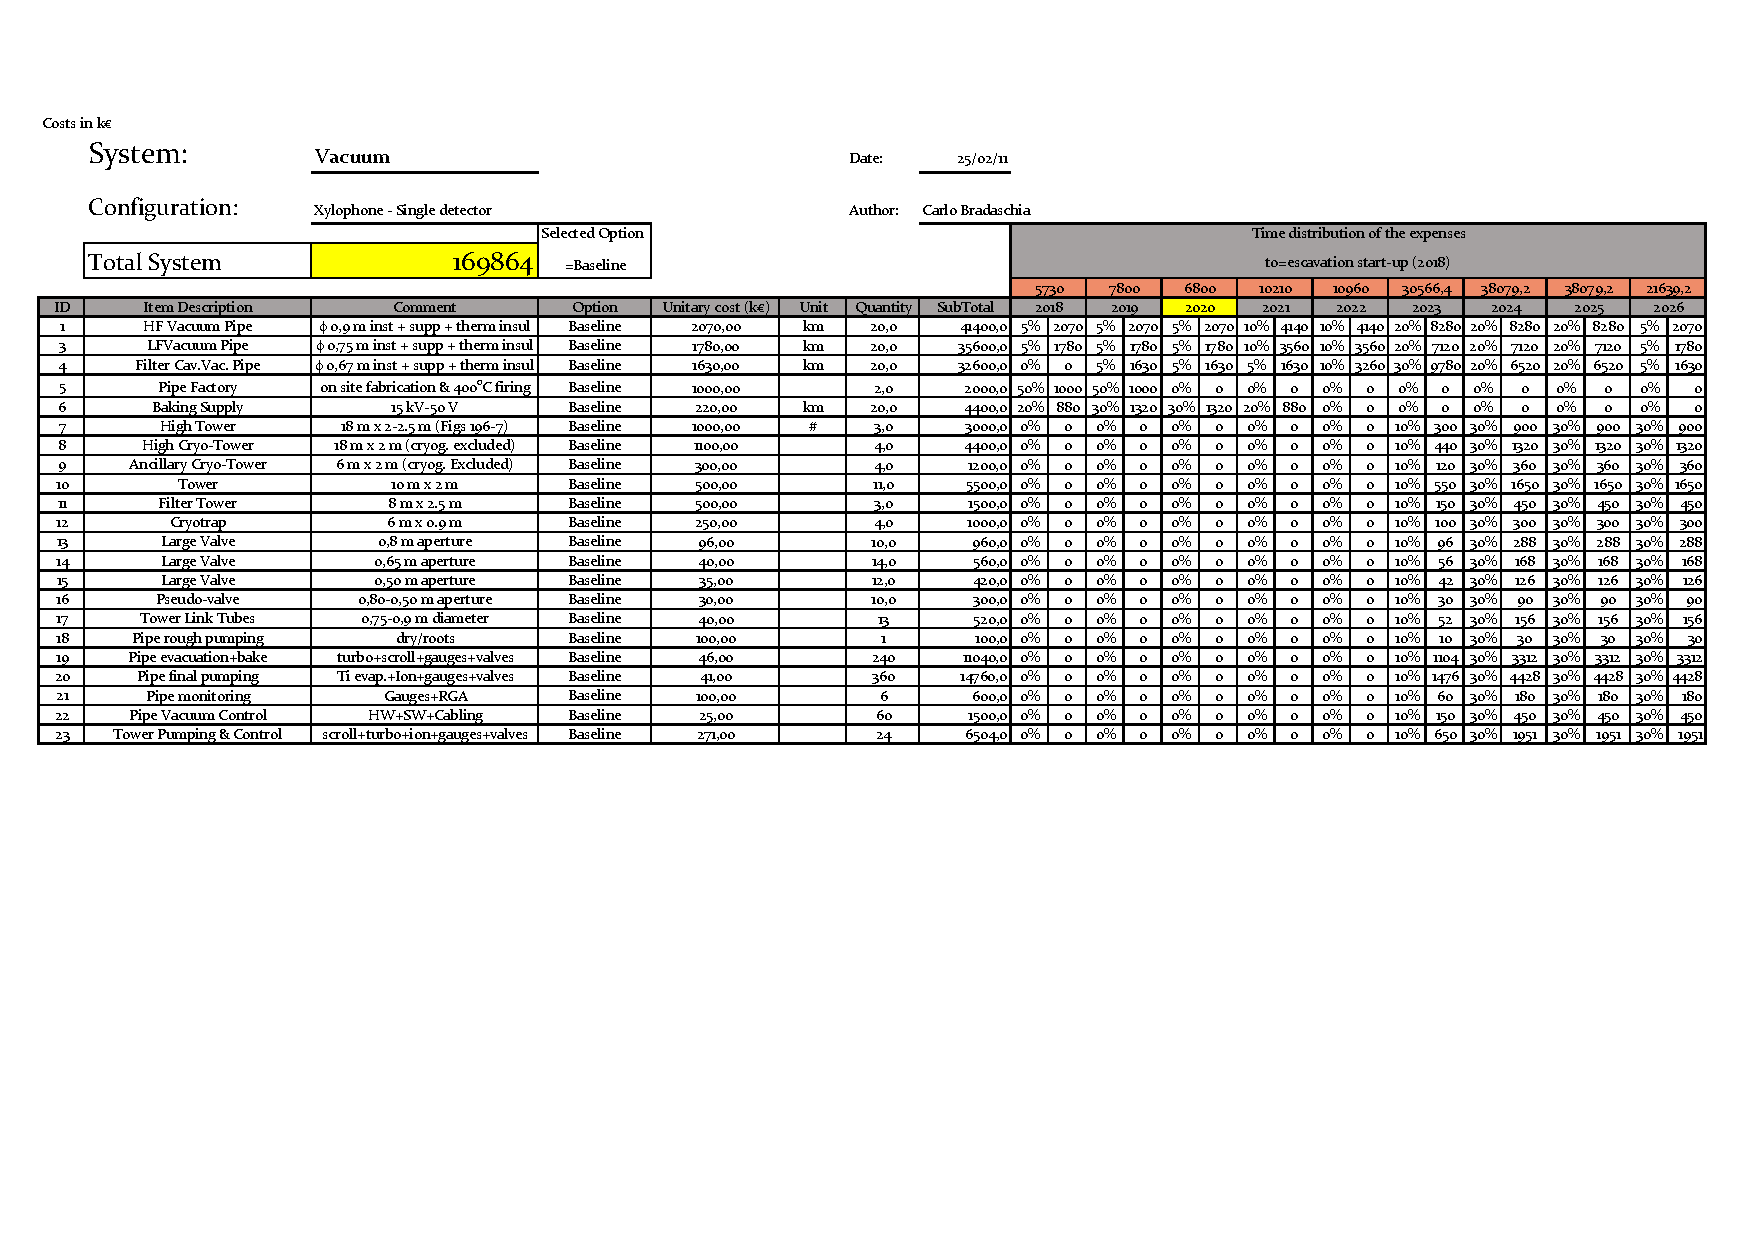
\includegraphics[angle=90, width=0.5\textwidth]{Sec_Conclusions/ET-cost-v00r05-Vacuum.pdf}
%\includegraphics[angle=90, width=0.5\textwidth]{Sec_Conclusions/ET-cost-v00r02.pdf}
%\includegraphics[width=0.49\textwidth, bb=0 0 800 600]{ET-B.png}
\caption{Vacuum apparatuses and components cost summary and expenditure time distribution}
\label{Fig:VacuumCostTable}
\end{figure}
%
\subsubsection[Cryogenics costs]{Cryogenic facilities and apparatuses cost preliminary evaluation}
%  
\label{ConclusionsCryoCostsSubSection}
%
This part of the cost evaluation is based both on the experience of previous experiments and on preliminary evaluations by some external company.
\par  
A rough evaluation of the cost of the cryostat is based on the experience gained in the construction of the cryogenic apparatus for the resonant gravitational wave detectors EXPLORER and NAUTILUS.
The cost of the nitrogen cryotraps is based on the Virgo experience. For the helium trap case we thank the CRIOTEC company, which helped us  in  the process of the cost assessment.
The cost of the cryogenic solution based on extensive use of cryo-coolers (see Fig.~\ref{Fig:CryoCoolerCostTable}) is based on the price market of such apparatuses made by the companies CRYOMECH (\url{http://www.cryomech.com/}, US) and  Sumitomo (\url{http://www.shicryogenics.com/}, Japan).
\par 
For the cryogenic solution based on extensive use cryo-fluids the economics of 4.5 K refrigeration, cryo-distribution and storage systems have been evaluated.
The experience gathered at CERN with the LEP~\cite{Kuhn1994467} and LHC projects~\cite{PhilippeLebrunMatefu}, which have \emph{de facto} turned the laboratory into a major world cryogenic center, has been considered. The recovered information have been updated taking into the account the price inflation of the Swiss currency. Then, this evaluation has been compared to that one performed for the cryogenic system planned for the International Linear Collider~\cite{ILCTomPeterson} and the educated guess done by the consulted experts of the Linde Kryotechnik~AG (\url{http://www.linde-kryotechnik.ch}, Switzerland).
The investment needed for the construction and the installation of the long flexible lines for the liquid helium transfer has been quoted, following the approach proposed in the CERN document~\cite{Kuhn:410808,Kuhn1994467,Claudet:410378,PhilippeLebrunMatefu} for LHC, which is based on the evaluation of the multiplication factors to scale the present cost of stainless steel piping. They  include engineering, installation and test  costs of the transfer lines. The rough cost evaluation, using extensively cryogenic fluids, is about 18 millions of Euro. 
%
\FloatBarrier
\begin{figure}[h]
\centering 
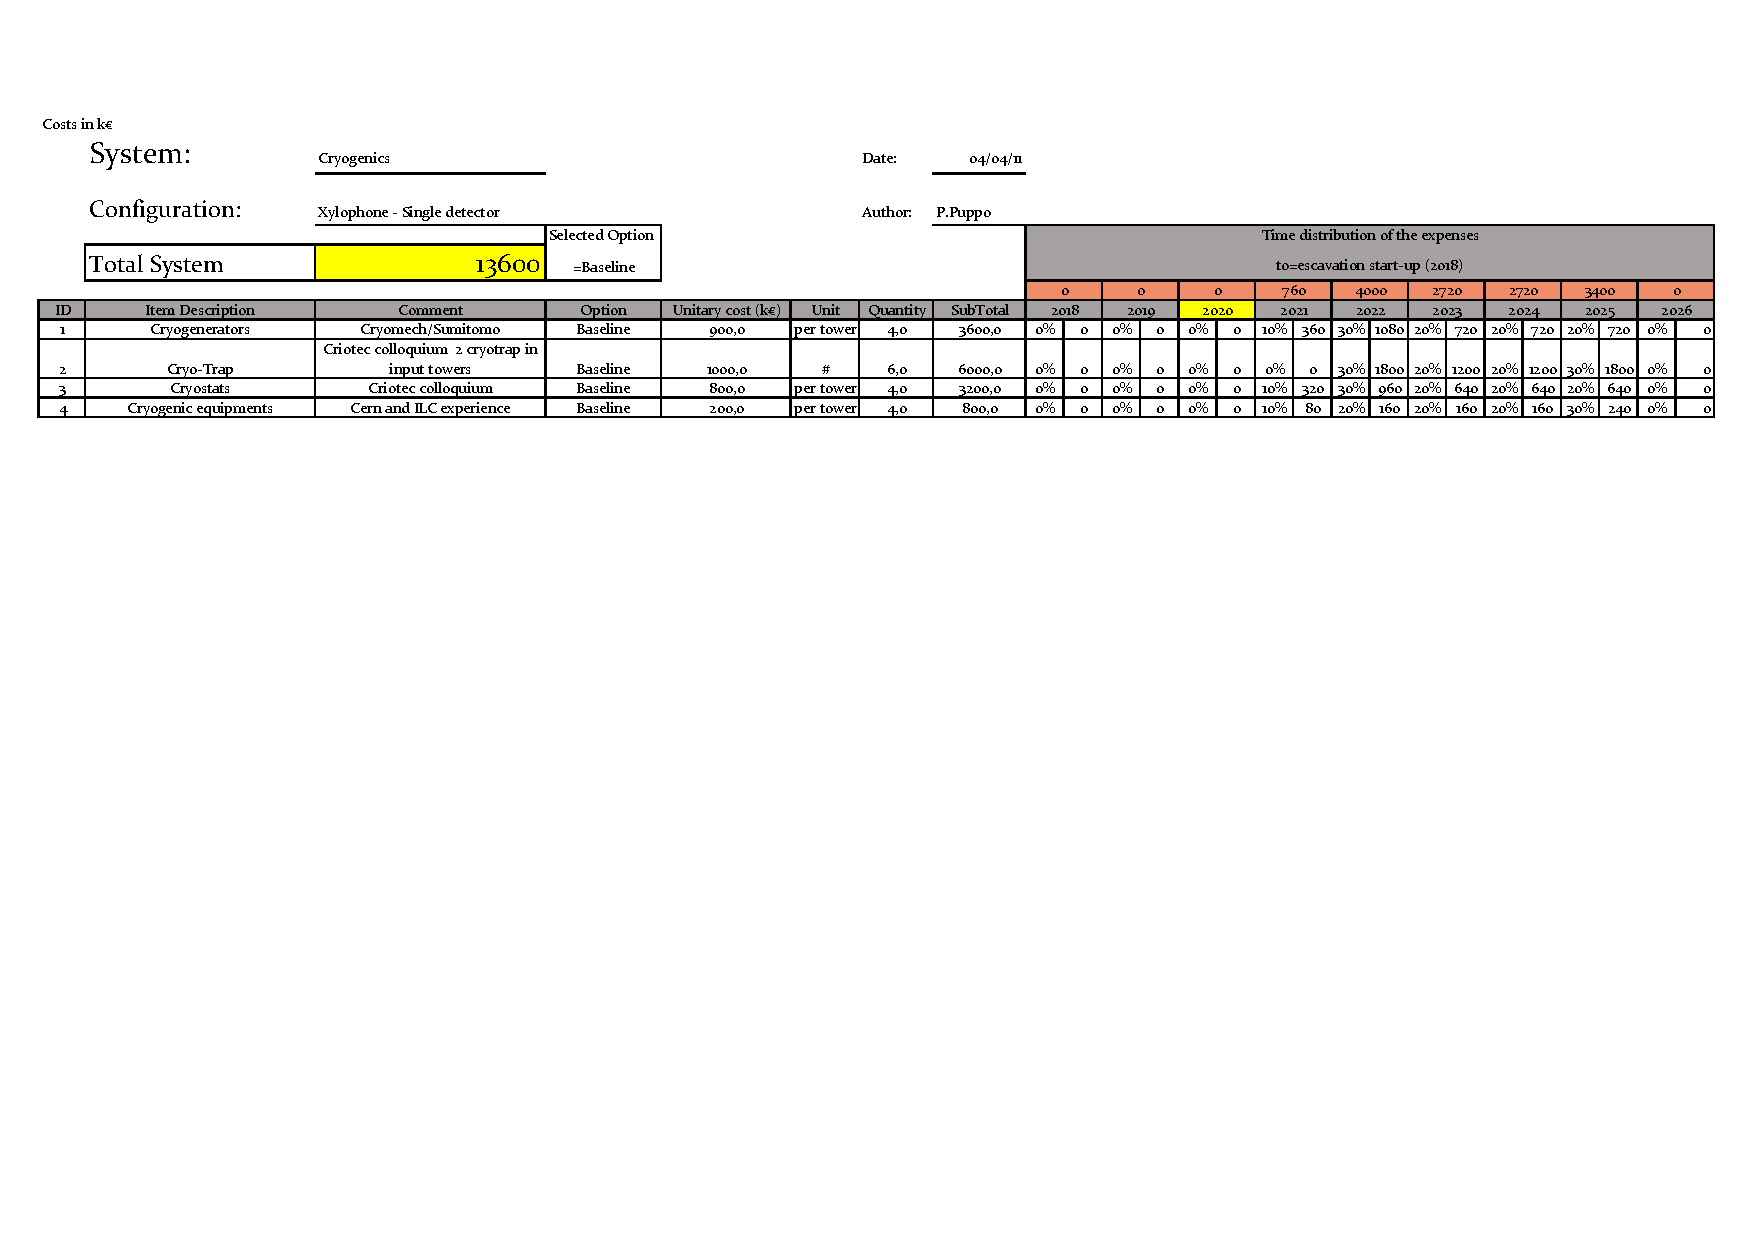
\includegraphics[angle=90, width=0.25\textwidth]{Sec_Conclusions/ET-cost-v00r04-CryoCoolers.pdf}
%\includegraphics[angle=90, width=0.5\textwidth]{Sec_Conclusions/ET-cost-v00r02.pdf}
%\includegraphics[width=0.49\textwidth, bb=0 0 800 600]{ET-B.png}
\caption{Cryo-coolers based solution cost summary and expenditure time distribution}
\label{Fig:CryoCoolerCostTable}
\end{figure}

%
%
\subsubsection[Suspensions costs]{Suspensions and payloads cost preliminary evaluation}
%  
\label{ConclusionsSuspCostsSubSection}
%
The cost evaluation for the payloads and the local control is based on the experience acquired during the construction of the Virgo monolithic suspensions and during the realisation of a cryogenic payload prototype built on Virgo site. In both cases the the mirrors have a mass of 20kg. 
For this reason we have newly evaluated the costs of the materials for building heavier and, in the ET-LF case, cryo-compatible  payload elements. 
In the case of the ET-LF interferometer the costs of the equipment for the temperature monitor with thermometers were added.
%
\FloatBarrier
\begin{figure}[h]
\centering 
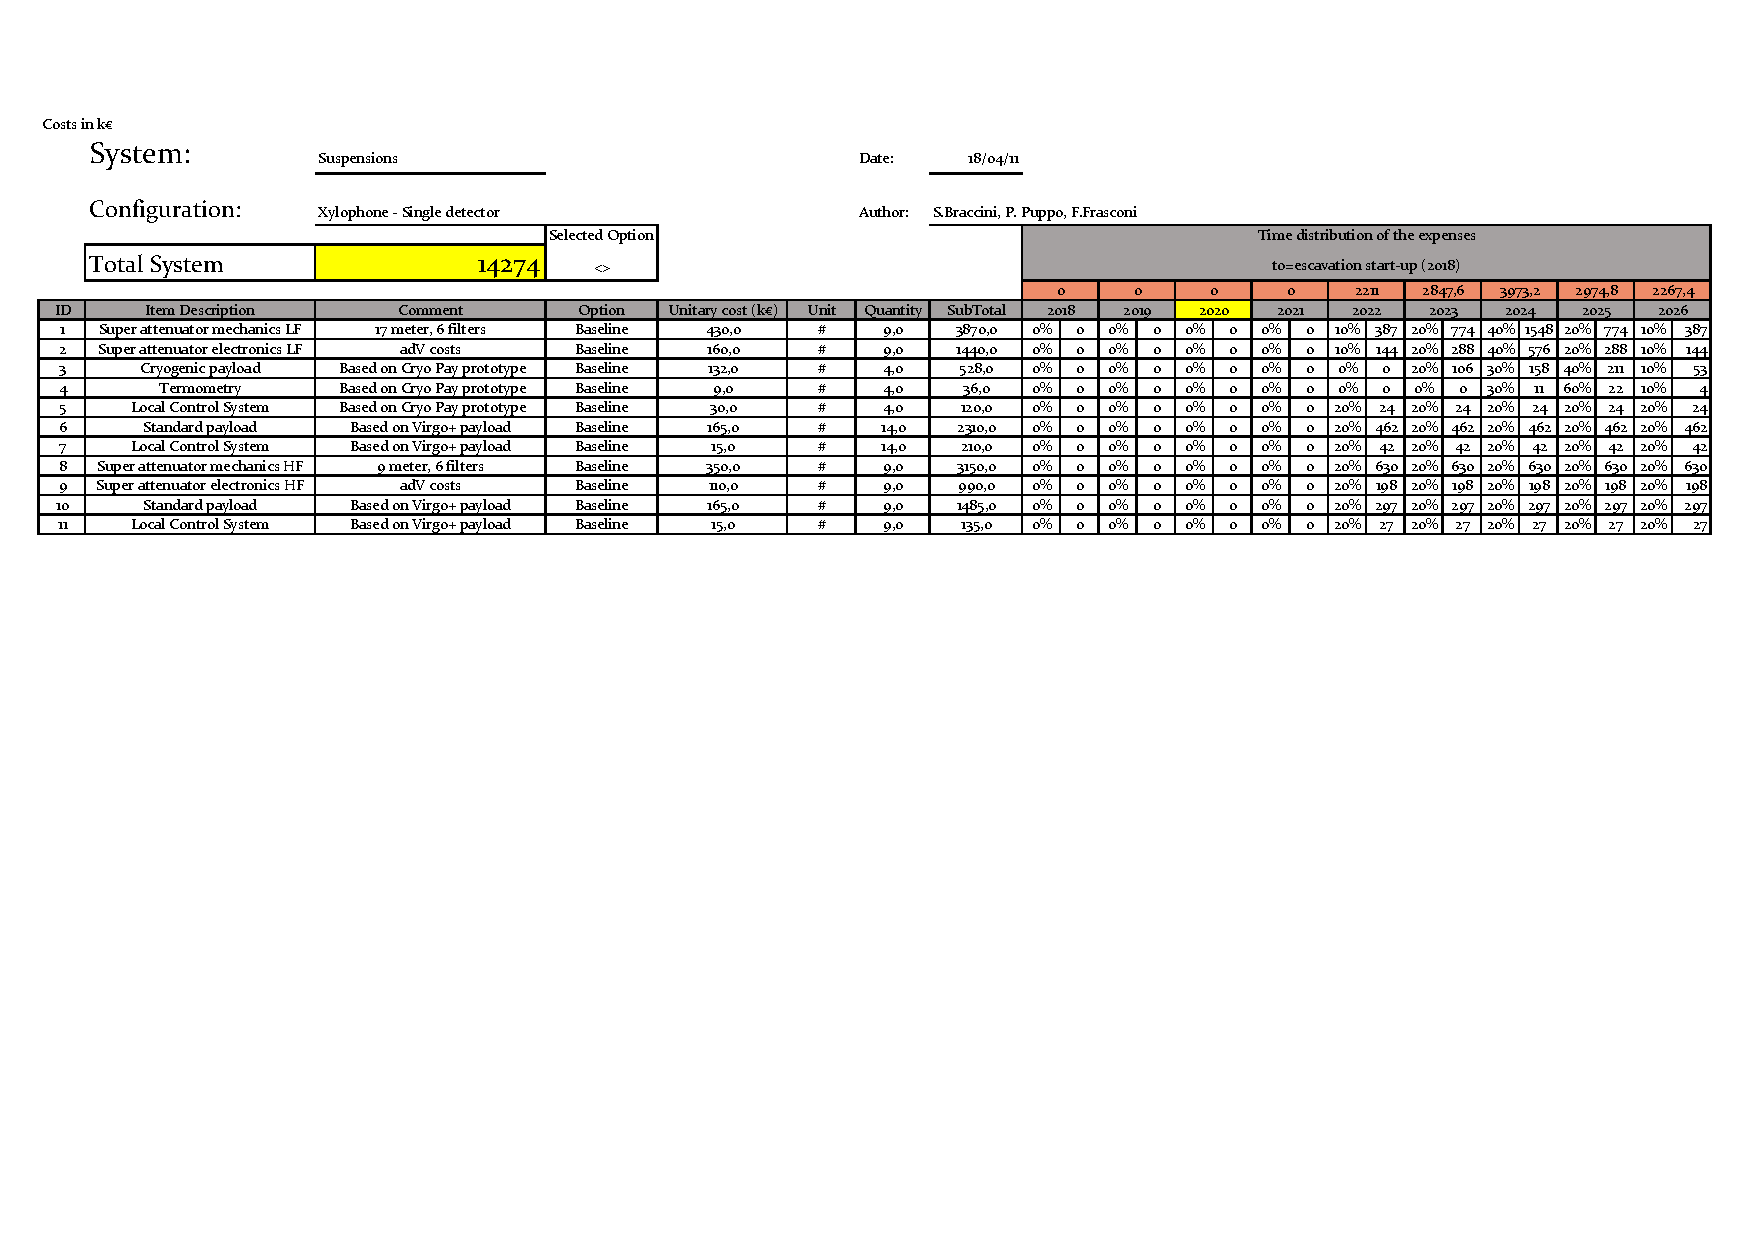
\includegraphics[angle=90, width=0.25\textwidth]{Sec_Conclusions/ET-cost-v00r05-Suspensions.pdf}
%\includegraphics[angle=90, width=0.5\textwidth]{Sec_Conclusions/ET-cost-v00r02.pdf}
%\includegraphics[width=0.49\textwidth, bb=0 0 800 600]{ET-B.png}
\caption{Suspensions cost summary (first detector) and expenditure time distribution}
\label{Fig:SuspensionsCostTable}
\end{figure}

%
%
\subsubsection[Optics costs]{Optics cost preliminary evaluation}
%  
\label{ConclusionsOpticsCostsSubSection}
%
% the file Opti_cost.tex is inserted both here and in the Optics.tex file
%
%
% this file is inserted through \input both in the Optics.tex and in the Conclusion.tex files
%
%\emph{Author(s): \textbf{A.\ Freise and H.\ Lueck} \\}
The main impact of the optical design on the cost is via the required infrastructure in terms of the vacuum system,
tunnels and caverns. In addition the optical system yields direct costs 
for the high-quality optics and the auxiliary optical systems with their mechanical and electrical support systems
The core elements of the interferometers are the test masses which need to be of considerable size and weight 
and must fulfil extremely stringent requirement for bulk and surface qualities.

The maximum available size for Suprasil~3001 today is the size of the 40\,kg test masses for advanced LIGO. The heavier 
substrates envisaged for ET can presently only be made either of Suprasil~3002 which has inhomogeneities in the direction of the 
beam or from fused pieces of thinner Suprasil~3001. The price quoted by Heraeus for a substrate of 600\,mm in diameter 
and 400\,mm in thickness made of composite Suprasil~3001 is \euro700k which corresponds approximately to a 
price of \euro3.5k/kg. The end test masses can be made out of Suprasil 312 with a considerable lower cost per kilogramme,
an estimate based on quotes for Advanced Virgo optics gives \euro1.6k/kg.

At present silicon is only available in Chzochalski grown crystals to a size of up to 450\,mm.%, the maximum resistance available for this type is ???
In Floating zone crystals the maximum size at present is 200\,mm. The interest of the semiconductor industry in ultra-pure crystals is 
very limited and will most likely not drive the development of bigger size single crystals.
Costs of silicon per kg are based on a quote by Simat and are comparable to the one of ultra-pure fused silica.

The cost estimates for polishing and coating of the mirrors are based on similar costs related to Advanced Virgo, up-scaled
to include ion-beam polishing.

Further included in the optics cost are the main laser systems, optical benches in air and in vacuum for injecting the beam from the laser
into the detectors, similar benches and components for extracting and detecting beams from the interferometers as well as
the mechanical, optical and electronic components required for interferometer control purposes. We further count the
cost for special optical subsystems such as the squeezed light source and the thermal compensation systems. These systems
will be directly based on current systems and thus the costs have been estimated from the data for current and advanced 
detectors.

The total cost for the installation of the optical components of the first detector (two interferometers plus spares) has
been computed as \euro37.6M. The total optics cost for all three detectors is estimated to be \euro60M. The nonlinear increase results
from the fact that spare parts can be shared between detectors. The cost of the first detector is dominated by the main
optics which account for \euro20.4M. The high-power laser system at 1064\,nm and one medium power system at 1550\,nm
wavelength cost together \euro7M. The input and output optics require together another \euro7M. We also include 
\euro2.5M for control electronics and \euro600k for the thermal compensation system.

%
\FloatBarrier
\begin{figure}[h]
\centering 
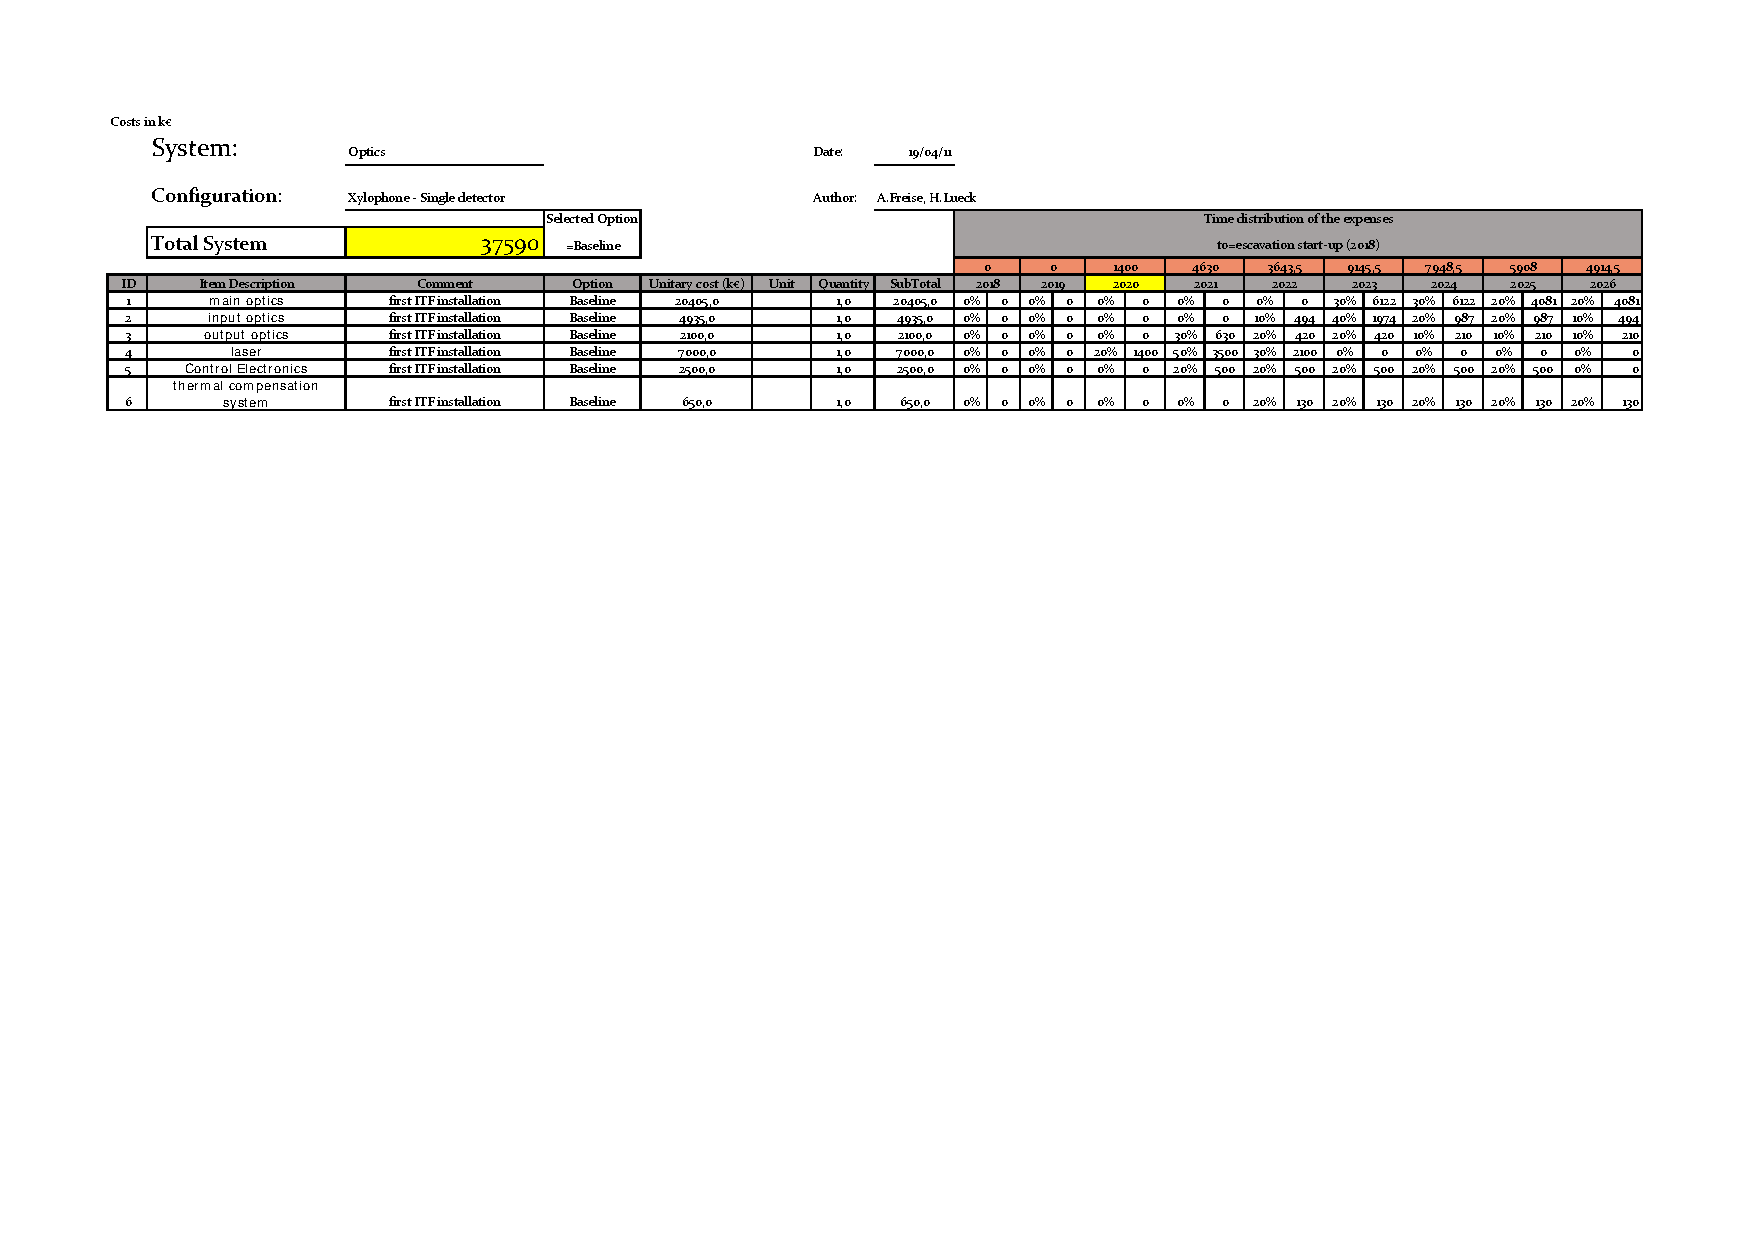
\includegraphics[angle=90, width=0.25\textwidth]{Sec_Conclusions/ET-cost-v00r05-Optics.pdf}
%\includegraphics[angle=90, width=0.5\textwidth]{Sec_Conclusions/ET-cost-v00r02.pdf}
%\includegraphics[width=0.49\textwidth, bb=0 0 800 600]{ET-B.png}
\caption{Optics cost summary (first detector) and expenditure time distribution}
\label{Fig:OpticsCostTable}
\end{figure}

